\documentclass[11pt]{article}
\usepackage[margin=1in]{geometry}
\usepackage{amsmath}
\usepackage{mathptmx}
\usepackage[T1]{fontenc}
\usepackage{booktabs}
\usepackage{pgfplots}
\pgfplotsset{compat=1.17}
\usepackage{caption}
\captionsetup{font=small}
\setlength{\parskip}{3pt}

\pgfplotsset{
  perf/.style={
    width=0.97\linewidth, height=5.4cm, grid=major,
    tick label style={font=\scriptsize}, label style={font=\small},
    legend style={font=\scriptsize, cells={anchor=west}},
    every axis plot/.append style={thick}
  },
  intervals/.style={
    symbolic x coords={0,5,10,20,50,100,200}, xtick=data,
    cycle list={{blue,mark=*},{red,mark=square*},{brown!80!black,mark=triangle*},{black,mark=star},{teal,mark=diamond*}},
    xlabel={Configured interval between moves (ms)}
  }
}

\title{COMP 512 Project 2 -- Performance Analysis of the Paxos Total-Order Layer}
\author{Group 19}
\date{}

\begin{document}
\maketitle
\vspace{-1.5em}

\section{Test Setup and Methodology}

\textbf{Implementation under test.} Every move is ordered by its own Paxos instance (\emph{slot}): the proposer sends \textsc{prepare} to all $n$ processes, waits for a majority of promises, sends \textsc{accept}, waits for a majority of acceptances, and broadcasts \textsc{decide}. There is no stable leader; each process proposes its own moves for the lowest slot it has not seen decided. A ballot is (\emph{counter}, \emph{process id}), where a new counter is the highest seen plus one and ties are ordered by process id. A refused proposer backs off for a random time in $[1, 5\cdot2^{k}]$\,ms ($k$ = consecutive failures, capped at 6) and retries. \texttt{broadcastTOMsg} blocks until a majority accepted, so each process has at most one outstanding move.

\textbf{Environment and experiments.} We used the provided \texttt{TreasureIslandAppAuto}, started by a parameterised copy of \texttt{run\_tiapp\_auto.sh}, with all $n$ processes on one host (Apple M3, 8 cores, 16\,GB, macOS, OpenJDK 21; GCL over loopback TCP; default \texttt{FINE} logging; sleep disabled with \texttt{caffeinate}). (A) $n\in\{2,3,5,7,9\}$ $\times$ interval $\in\{0,5,10,20,50,100,200\}$\,ms, 150 moves per player, 2 repetitions with different seeds (70 runs). (B) Fairness: $n\in\{5,9\}$, interval 0, 200 moves per player, 5 repetitions (10 runs). In all 80 runs all island logs were identical and contained every move of every player.

\textbf{Metrics.} \emph{Latency} is the time from the call to \texttt{broadcastTOMsg} until a majority has accepted the move, taken from our log timestamps; the first 5 moves of each player (connection set-up, JIT warm-up) are excluded. \emph{System throughput} is the number of decided slots per second at player~1 between the 10th and 90th percentile of decision times, which excludes start-up and the tail where some players have finished. The \emph{per-process acceptance rate} is a player's number of moves divided by the time from its first broadcast to its last acceptance. The provided move generator sleeps until \emph{interval} ms have passed since its last move, but \texttt{Thread.sleep} overshoots by $\approx$2\,ms on our machine (median gap 12.2\,ms at a 10\,ms setting, while Paxos took $\approx$1\,ms). Each process therefore offers at most $1000/(\text{interval}+2)$ moves/s.

\section{Impact of the Number of Players and the Interval}

\textbf{Latency (Fig.~\ref{fig:lat}).} With large intervals (100--200\,ms) moves of different players rarely overlap and latency is 4--9\,ms for every $n$: the cost of one uncontested instance, i.e.\ two round trips to a majority over loopback plus synchronous logging of every GCL message. As the interval shrinks, latency grows, and faster the more players there are: at 20\,ms it is 2.6\,ms for $n=2$ but 32\,ms for $n=9$, and at interval 0 it reaches 41\,ms (p95 200\,ms) for $n=9$. The cause is contention: several players propose for the same slot, only one wins, and the others are refused, back off and retry. Fig.~\ref{fig:max}(b) shows this directly: the number of rounds per committed move rises from 1.1--1.5 at 200\,ms to 4.6 for $n=9$ at interval 0, and every lost round adds a round trip plus a random backoff. Each round also costs $\approx5n$ messages and all $n$ JVMs share 8 cores, so rounds themselves get slower as $n$ grows. For $n=2$, latency at 50--200\,ms (4.2--5.1\,ms) is higher than at 10--20\,ms (2.5\,ms). We attribute this to the processes idling between moves, so threads must be woken and the CPU leaves its low-power state for each move.

\textbf{Throughput (Fig.~\ref{fig:thr}).} For large intervals the system is not the bottleneck: throughput equals the offered load $n\cdot1000/(\text{interval}+2)$ (e.g.\ 43.7 moves/s for $n=9$ at 200\,ms, 4.9 per player), so it grows linearly with $n$ and inversely with the interval. As the interval decreases, the curves stop following the offered load and flatten. This happens earlier for more players, because their offered load is higher and their capacity, limited by contention, is lower: $n=9$ reaches its plateau of $\approx$180--195 moves/s already at 20\,ms, $n=7$ stays at 210--250 moves/s for 5--20\,ms, while $n=2$ follows the offered load down to 5\,ms.

\section{Fairness Between Processes}

At large intervals all processes have the same acceptance rate (4.8--4.9 moves/s each at 200\,ms), because every move is accepted long before the next one is generated. As the interval approaches 0 this changes (Fig.~\ref{fig:fair}): the acceptance rate shows a clear upward trend with the process number in every repetition. With 5 players, process~5 is accepted 34\% more often than process~1 (97.4 vs.\ 72.7 moves/s; mean latency 7.9 vs.\ 10.3\,ms), and process~1 was the slowest in all 5 repetitions. With 9 players, processes~8 and~9 are $\approx$23\% faster than process~1 (25.0 vs.\ 20.4 moves/s), and one of them was the fastest process in every repetition.

The responsible aspect of our algorithm is the ballot tie-break. Every proposer picks ``highest counter seen + 1'', so proposers starting at about the same time usually choose the \emph{same} counter, and the tie is decided by the process id. Our ids are \texttt{host:port} with ports increasing with the player number, so a higher player always wins a tie. Table~\ref{tab:tie} confirms this from the acceptor logs of a separate 5-player run: process~5 received no tie refusals while process~1 received 382, and process~1 lost 3.8 times as many phase-1 rounds as process~5. Each lost tie costs the loser a refusal, a backoff and a retry. The randomised backoff and the adoption of the highest counter seen keep the bias bounded: no process starves. It could be removed by breaking ties with a random per-ballot number or rotating the tie-break priority with the slot number.

\section{Maximum Throughput}

Fig.~\ref{fig:max}(a) shows the throughput at interval 0, where every player re-proposes as soon as its previous move is accepted. The maximum is $\approx$585 moves/s with 2 players, $\approx$490--510 with 3 and 5 players (large variance for $n=5$: 357--610 over 7 runs), and drops to $\approx$287 with 7 and $\approx$206 with 9 players. The rate does not need to reach interval 0 to flatten out: for $n=9$, 5--20\,ms already yield 180--195 moves/s, the same as interval 0, and for $n=7$ the plateau starts at 10--20\,ms. Only for $n=2,3$ does the curve keep rising down to 0, because even at 5\,ms each player still sleeps $\approx$7\,ms after each fast move, so throughput is limited by the offered load, not by Paxos. The maximum falls as players are added because (i) every instance needs $\approx5n$ messages, (ii) contention grows (4.6 rounds per move at $n=9$ vs.\ 1.3 at $n=2$, each lost round adding a backoff), and (iii) all players share one machine (8 cores, $n$ JVMs, synchronous logging). A stable leader that pipelines moves would avoid most collisions, but the assignment requires each process to propose its own moves.

\textbf{Limitations.} All numbers come from a single host over loopback; on the SOCS machines network round trips would add to every latency and change the share of time lost to contention.

%========================= FIGURES =========================
\clearpage

\begin{figure}[t]
\centering
\begin{minipage}{0.49\linewidth}
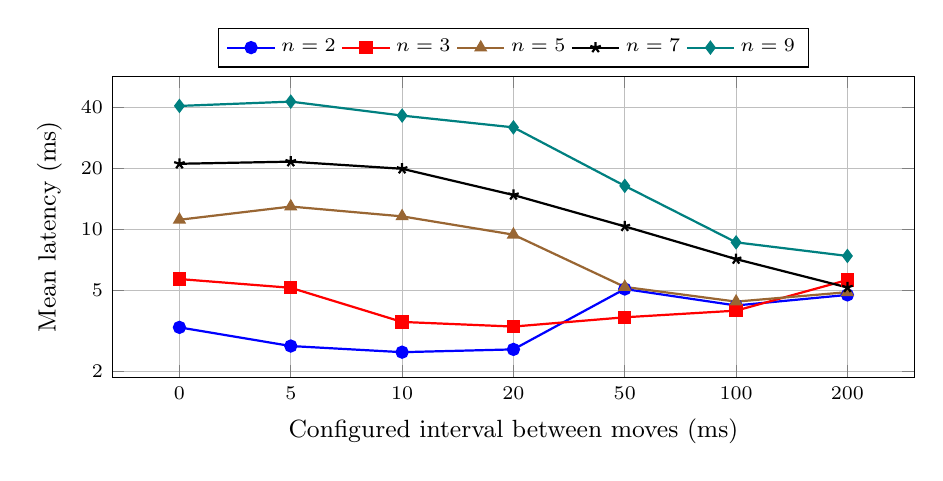
\begin{tikzpicture}
\begin{axis}[perf, intervals, ymode=log, log ticks with fixed point, ytick={2,5,10,20,40}, ylabel={Mean latency (ms)}, legend style={at={(0.5,1.03)}, anchor=south, legend columns=5, font=\scriptsize}]
\addplot coordinates {(0,3.30) (5,2.67) (10,2.49) (20,2.57) (50,5.10) (100,4.23) (200,4.77)};
\addplot coordinates {(0,5.71) (5,5.17) (10,3.51) (20,3.33) (50,3.70) (100,3.99) (200,5.65)};
\addplot coordinates {(0,11.19) (5,13.00) (10,11.63) (20,9.45) (50,5.22) (100,4.42) (200,4.92)};
\addplot coordinates {(0,21.12) (5,21.64) (10,19.96) (20,14.82) (50,10.38) (100,7.16) (200,5.19)};
\addplot coordinates {(0,40.72) (5,42.76) (10,36.50) (20,31.93) (50,16.44) (100,8.66) (200,7.42)};
\legend{$n=2$,$n=3$,$n=5$,$n=7$,$n=9$}
\end{axis}
\end{tikzpicture}
\end{minipage}\hfill
\begin{minipage}{0.49\linewidth}
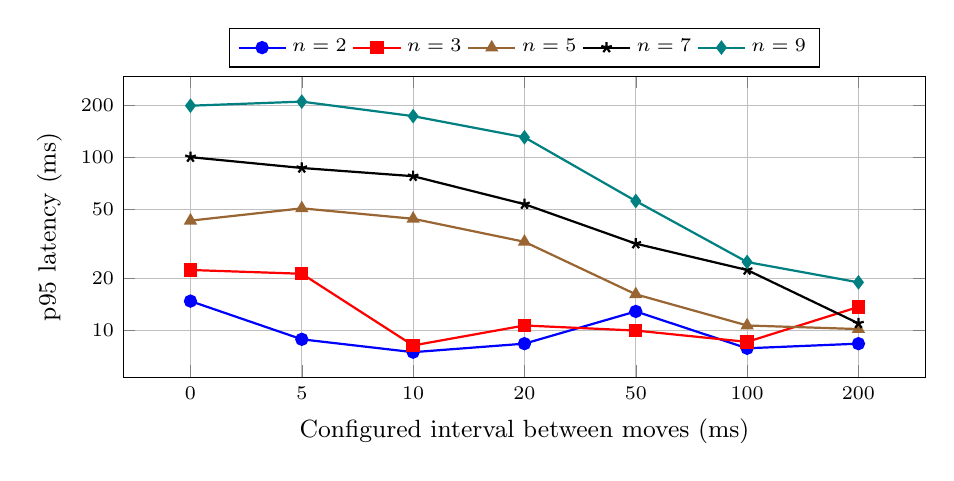
\begin{tikzpicture}
\begin{axis}[perf, intervals, ymode=log, log ticks with fixed point, ytick={5,10,20,50,100,200}, ylabel={p95 latency (ms)}, legend style={at={(0.5,1.03)}, anchor=south, legend columns=5, font=\scriptsize}]
\addplot coordinates {(0,14.8) (5,8.9) (10,7.5) (20,8.4) (50,12.9) (100,7.9) (200,8.4)};
\addplot coordinates {(0,22.4) (5,21.3) (10,8.2) (20,10.7) (50,10.0) (100,8.6) (200,13.7)};
\addplot coordinates {(0,43.2) (5,50.9) (10,44.3) (20,32.6) (50,16.2) (100,10.7) (200,10.2)};
\addplot coordinates {(0,100.6) (5,87.1) (10,78.1) (20,53.8) (50,31.8) (100,22.4) (200,11.0)};
\addplot coordinates {(0,199.6) (5,210.7) (10,173.7) (20,131.0) (50,56.1) (100,24.9) (200,19.0)};
\legend{$n=2$,$n=3$,$n=5$,$n=7$,$n=9$}
\end{axis}
\end{tikzpicture}
\end{minipage}
\caption{Time until a move is accepted (from \texttt{broadcastTOMsg} until a majority accepted it) vs.\ the configured interval, for $n$ players. Left: mean; right: 95th percentile (both log scale; mean of 2 repetitions, 150 moves per player).}
\label{fig:lat}
\end{figure}

\begin{figure}[t]
\centering
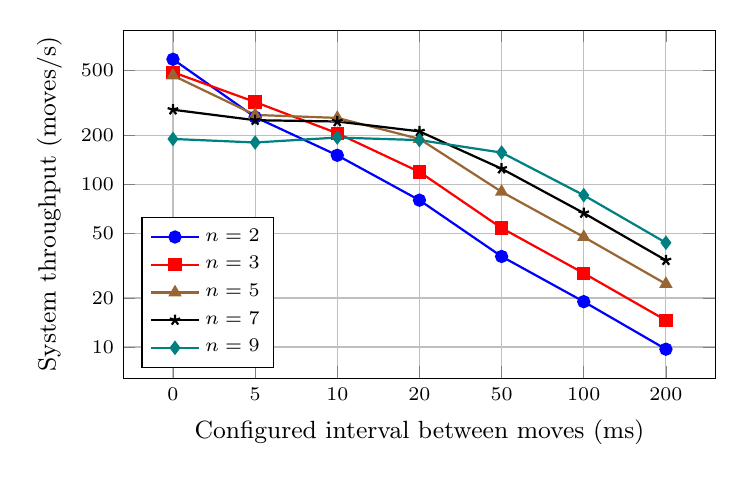
\begin{tikzpicture}
\begin{axis}[perf, intervals, width=0.75\linewidth, height=6cm, ymode=log, log ticks with fixed point, ytick={10,20,50,100,200,500}, ylabel={System throughput (moves/s)}, legend pos=south west]
\addplot coordinates {(0,585.1) (5,258.4) (10,150.5) (20,79.8) (50,36.0) (100,19.0) (200,9.7)};
\addplot coordinates {(0,487.3) (5,319.8) (10,205.6) (20,119.0) (50,53.8) (100,28.4) (200,14.6)};
\addplot coordinates {(0,465.0) (5,266.4) (10,255.4) (20,189.8) (50,89.8) (100,47.4) (200,24.4)};
\addplot coordinates {(0,286.7) (5,247.3) (10,242.7) (20,211.1) (50,124.5) (100,66.5) (200,34.1)};
\addplot coordinates {(0,189.7) (5,180.4) (10,193.5) (20,186.6) (50,156.4) (100,85.6) (200,43.7)};
\legend{$n=2$,$n=3$,$n=5$,$n=7$,$n=9$}
\end{axis}
\end{tikzpicture}
\caption{Moves decided per second by the whole system vs.\ the configured interval (log scale; mean of 2 repetitions). At large intervals the throughput equals the offered load $n\cdot1000/(\text{interval}+2)$; at small intervals it flattens at the capacity of the system, which decreases as $n$ grows.}
\label{fig:thr}
\end{figure}

\begin{figure}[t]
\centering
\begin{minipage}{0.49\linewidth}
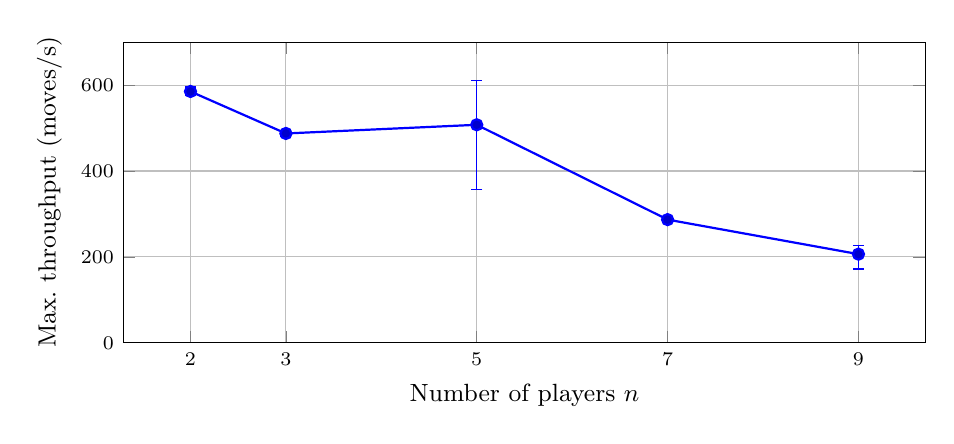
\begin{tikzpicture}
\begin{axis}[perf, xlabel={Number of players $n$}, ylabel={Max.\ throughput (moves/s)}, xtick={2,3,5,7,9}, ymin=0, ymax=700]
\addplot+[mark=*, error bars/.cd, y dir=both, y explicit] coordinates {
  (2,585.1) += (0,10.3) -= (0,10.3)
  (3,487.3) += (0,7.6) -= (0,7.5)
  (5,507.5) += (0,102.2) -= (0,150.9)
  (7,286.7) += (0,7.5) -= (0,7.5)
  (9,206.3) += (0,20.8) -= (0,34.5)};
\end{axis}
\end{tikzpicture}
\end{minipage}\hfill
\begin{minipage}{0.49\linewidth}
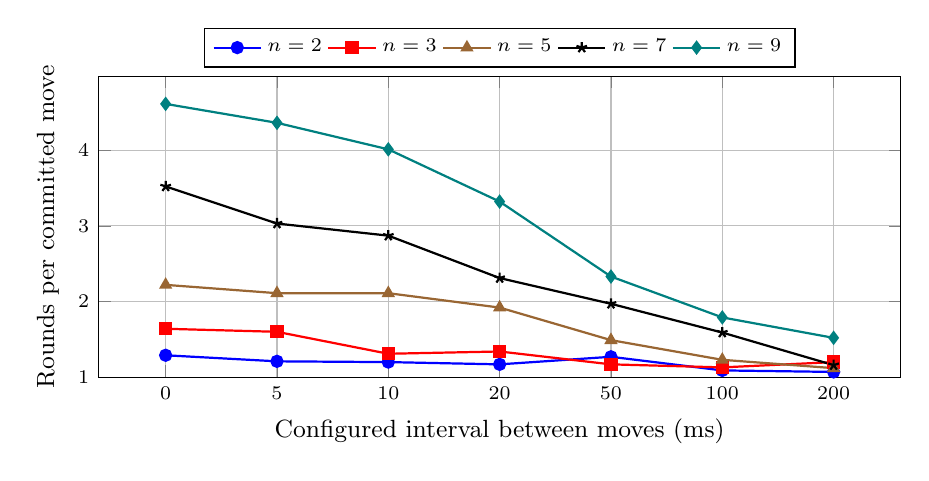
\begin{tikzpicture}
\begin{axis}[perf, intervals, ylabel={Rounds per committed move}, legend style={at={(0.5,1.03)}, anchor=south, legend columns=5, font=\scriptsize}, ymin=1]
\addplot coordinates {(0,1.29) (5,1.21) (10,1.20) (20,1.17) (50,1.27) (100,1.09) (200,1.07)};
\addplot coordinates {(0,1.64) (5,1.60) (10,1.31) (20,1.34) (50,1.17) (100,1.13) (200,1.20)};
\addplot coordinates {(0,2.22) (5,2.11) (10,2.11) (20,1.92) (50,1.49) (100,1.23) (200,1.12)};
\addplot coordinates {(0,3.52) (5,3.03) (10,2.87) (20,2.31) (50,1.97) (100,1.59) (200,1.16)};
\addplot coordinates {(0,4.61) (5,4.36) (10,4.01) (20,3.32) (50,2.33) (100,1.79) (200,1.52)};
\legend{$n=2$,$n=3$,$n=5$,$n=7$,$n=9$}
\end{axis}
\end{tikzpicture}
\end{minipage}
\caption{(a) Left: maximum throughput (interval 0) vs.\ number of players; mean with min/max over all runs (2 runs for $n=2,3,7$; 7 runs for $n=5,9$). (b) Right: contention, measured as the number of Paxos rounds started per committed move. 1.0 means every move succeeded in its first round.}
\label{fig:max}
\end{figure}

\begin{figure}[t]
\centering
\begin{minipage}{0.40\linewidth}
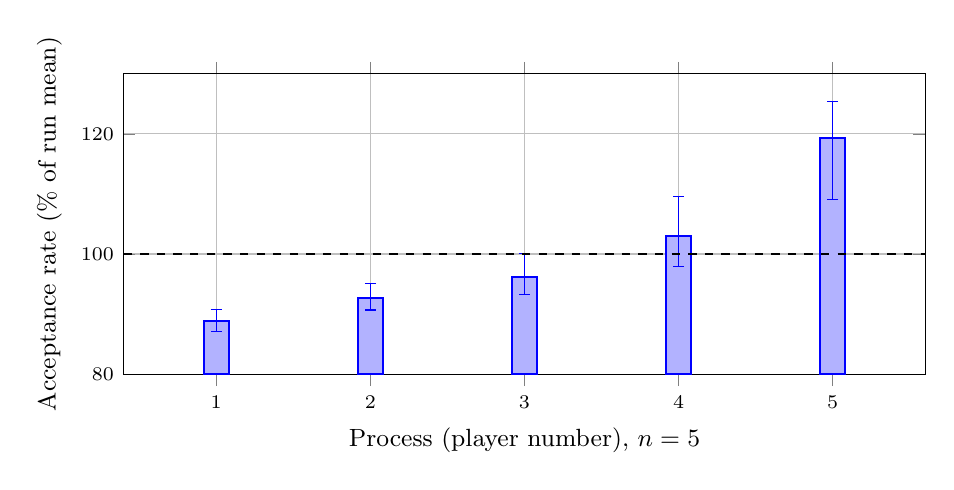
\begin{tikzpicture}
\begin{axis}[perf, ybar, bar width=9pt, xlabel={Process (player number), $n=5$}, ylabel={Acceptance rate (\% of run mean)}, xtick={1,2,3,4,5}, xmin=0.4, xmax=5.6, enlarge x limits=false, ymin=80, ymax=130]
\addplot+[error bars/.cd, y dir=both, y explicit] coordinates {
  (1,88.9) += (0,1.9) -= (0,1.8)
  (2,92.7) += (0,2.4) -= (0,2.0)
  (3,96.2) += (0,3.9) -= (0,2.9)
  (4,103.0) += (0,6.5) -= (0,5.1)
  (5,119.3) += (0,6.0) -= (0,10.2)};
\addplot[sharp plot, dashed, black, thin, domain=0.4:5.6, samples=2] {100};
\end{axis}
\end{tikzpicture}
\end{minipage}\hfill
\begin{minipage}{0.58\linewidth}
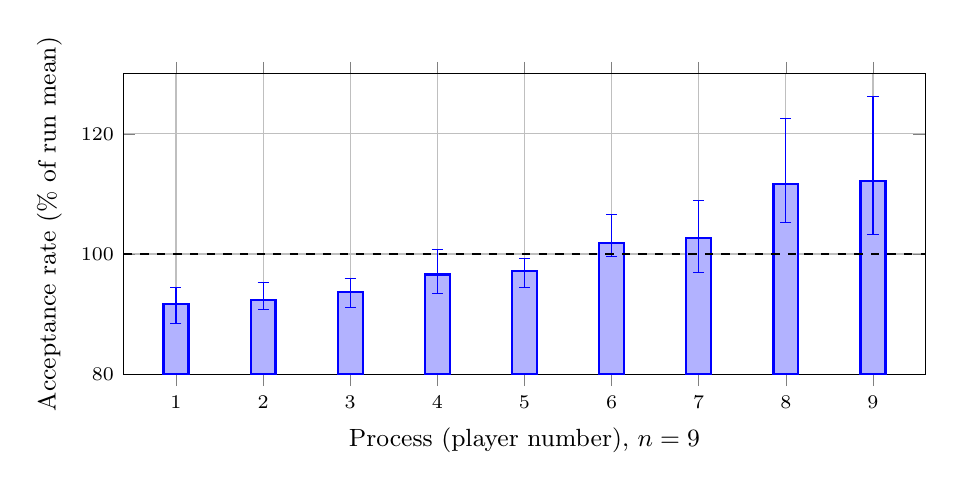
\begin{tikzpicture}
\begin{axis}[perf, ybar, bar width=9pt, xlabel={Process (player number), $n=9$}, ylabel={Acceptance rate (\% of run mean)}, xtick={1,2,3,4,5,6,7,8,9}, xmin=0.4, xmax=9.6, enlarge x limits=false, ymin=80, ymax=130]
\addplot+[error bars/.cd, y dir=both, y explicit] coordinates {
  (1,91.7) += (0,2.7) -= (0,3.2)
  (2,92.4) += (0,2.8) -= (0,1.6)
  (3,93.7) += (0,2.3) -= (0,2.6)
  (4,96.6) += (0,4.2) -= (0,3.2)
  (5,97.2) += (0,2.0) -= (0,2.7)
  (6,101.9) += (0,4.7) -= (0,2.3)
  (7,102.7) += (0,6.2) -= (0,5.8)
  (8,111.6) += (0,11.0) -= (0,6.4)
  (9,112.2) += (0,14.0) -= (0,8.9)};
\addplot[sharp plot, dashed, black, thin, domain=0.4:9.6, samples=2] {100};
\end{axis}
\end{tikzpicture}
\end{minipage}
\caption{Per-process acceptance rate at interval 0, relative to the mean of all processes in the same run (100\% = perfectly fair). Bars: mean of 5 repetitions; whiskers: min/max. Absolute means: 72.7--97.4 moves/s ($n=5$) and 20.4--25.0 moves/s ($n=9$).}
\label{fig:fair}
\end{figure}

\begin{table}[t]
\centering
\small
\begin{tabular}{lccccc}
\toprule
Process (player) & 1 & 2 & 3 & 4 & 5\\
\midrule
Refusals because of an equal-counter tie lost to a higher id & 382 & 301 & 320 & 187 & 0\\
Refusals because of a higher counter & 188 & 263 & 330 & 325 & 328\\
Rounds lost in phase 1 & 69 & 53 & 61 & 34 & 18\\
Rounds lost in phase 2 & 61 & 68 & 76 & 78 & 59\\
\bottomrule
\end{tabular}
\caption{Why the higher-numbered processes are faster: the causes of refusals received by each proposer, counted from all acceptors' logs of one 5-player run at interval 0 (200 moves per player). Process~5 has the highest id and never loses a tie.}
\label{tab:tie}
\end{table}

\end{document}
